%%% XeLaTeX-article %%%
%# -*- coding: utf-8 -*-
%!TEX encoding = UTF-8 Unicode
%!TEX TS-program = xelatex  
%---------------------虽然加了%还是要保留!

\documentclass[17pt]{beamer}
\mode<presentation>
{
\usetheme[width=40pt]{Hannover}
\usecolortheme[]{dove}
\usefonttheme[]{structurebold}
\setbeameroption{hide notes}
}

\usepackage{fontspec}
\setmainfont{Arial} %设置主字体
\newfontfamily\sanskritfont[Script=Devanagari,Mapping=romantodevanagari,Scale=1.15]{Sanskrit 2003}             %输出天城体
%\newfontfamily\sanskritfont[Mapping=tex-text]{Times New Roman}              %输出转写
\doublehyphendemerits=-10000
\newcommand{\skt}[1]{{\sanskritfont{#1}}} %输出天城体
\newcommand{\skttrans}[1]{{\skt{#1}~#1}}  %输出天城体和转写
%----------------------------------------------------设置梵文输入方法

\usepackage[UTF8,fontset=windows]{ctex}
\usepackage{amsmath}
\usepackage{xpinyin}
%----------------------------------------------------设置中文输入相关

\usepackage{graphicx}
\usepackage{flafter} 
\graphicspath{{pic/}}
\usepackage{booktabs}
 
%-----------------------------------------插图表格

\usepackage{hyperref} 
\hypersetup{
    colorlinks=true,
    linkcolor=black,
    urlcolor=blue
}
\usepackage{bookmark} 
%------------------------------目录结构


\title{{梵语入门}}
\subtitle{1. 课程介绍与字母}
\author[张雪杉]{文学院~~张雪杉 \\ zhangxueshan@sdnu.edu.cn}
\date{}
%\institute{}



\begin{document}	


\begin{frame}
  \titlepage
\end{frame}

\begin{frame}
  \frametitle{本节内容}
  \tableofcontents
\end{frame}

\section{课程介绍}

\begin{frame}{《故事海》}
    \centering
    \hspace*{-1cm} % Adjust the -1cm value to control the left shift    
    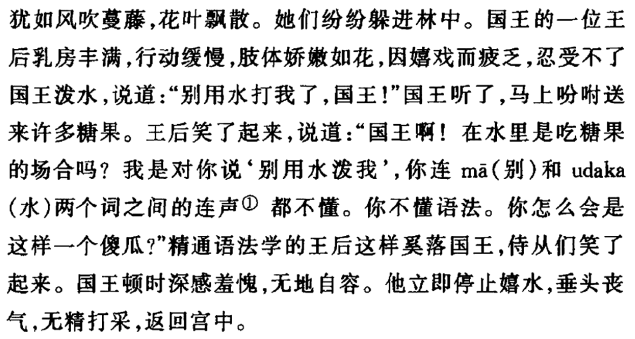
\includegraphics[width=0.67\textwidth]{satavahana1.png}
    \hspace*{1cm} % Adjust the 1cm value to control the right shift
    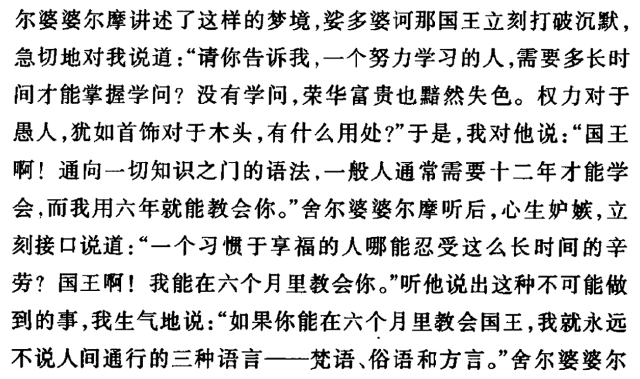
\includegraphics[width=0.67\textwidth]{satavahana2.png}
\end{frame}

\begin{frame}{\insertsection }
  \footnotesize
    \hspace*{2em}梵语(Sanskrit)是古印度文化的核心语言,广泛用于吠陀、史诗、佛教文献等经典,是学习印度哲学、文学和宗教的钥匙。本课程为从零开始的入门课,使用广受好评的教材\textit{The Cambridge Introduction to Sanskrit},英文教材中文讲授,涵盖该书前16章的内容,旨在初步打下语法、词汇和阅读基础。课程从天城体及转写体字母和发音规则开始,概述名词的性、数、格变化,动词的时态、语态及现在时系统变位,并引入复合词、分词等。每周上课两课时,包括语法教学与练习讲解,需要学生课外约两到三小时的预习准备,练习字母书写及短句翻译,尝试阅读《摩诃婆罗多》等经典文本中的句子。结课时学生能掌握基本语法,积累常用词汇,读写简单梵语句子,为“梵语提高”课程做好准备。
\end{frame}

\begin{frame}{期末作业}
  \scriptsize
  \raggedright
  \begin{verse}
    \skt{1) sukeśā kanyā gṛhamaviśatkumāraśca kṣaṇādadatiṣṭhat ।} \\
    \skt{2) nṛpāya natvā prajāstaṃ  cintāḥ kathayanti ।} \\
    \skt{3) grāmātpratyāgatya nārī priyāṃ nagarīṃ dṛṣṭvā kṣaṇātprāviśat ।} \\
    \skt{4) kṛtsnaṃ deśamabhibhūyogro nṛpo nagarīradahat ।} \\
    \skt{5) kva nagarīṇāṃ pālā bhavantīti nārī dagdhā nagarīrdṛṣṭvāpṛcchat ।} \\
    \mbox{\skt{6) naro bālāpālāṃ dāsīṃ varairdānaistoṣayitvā bālāṃ gṛhamanayat ।}} \\
    \mbox{\skt{7) bhīmau kṣatriyau narasya bhāryāṃ sabālāṃ luptvā naraṃ duḥkhamatyajatām ।}} \\
    \skt{8) nagaravananadīrdṛṣṭvā tuṣṭo bālo gṛhaṃ pratyāgacchat ।} \\
    \skt{9) bālo vismayena rājñyā ratnāni dṛṣṭvā tasyāḥ  prabhā sūryasyeveti cintayati ।} \\
  \end{verse}
\end{frame}


\subsection{课程平台}
\begin{frame}{\insertsubsection }
  \begin{itemize}
    \item
      课程网站:超星学习通 \\
      = 学校主页\nobreakdash-信息门户\nobreakdash-慧课慧学
    \item
      课程邀请码:1855857
  \end{itemize}
\end{frame}

\subsection{教材与参考资料}
\begin{frame}{\insertsubsection }
  \begin{itemize}
    \item
      教材: \textit{The Cambridge Introduction to Sanskrit}
    \item
      中文参考书:《梵文基础读本》
    \item
      资料:课件、教材勘误表、习题参考答案等, \href{http://yun.sdnu.edu.cn/\#/link/CCAB068CE5DFF94EAACB1A221F2D3B9B}{共享文件夹}查看更多 
  \end{itemize}
\end{frame}

\subsection{考核方式}
\begin{frame}{\insertsubsection }
  \begin{itemize}
    \item
      平时20分:课后问卷15*3\\ 上课需轮流做作业题~~但不好算分
    \item
      期中30分:默写字母表\\第九周左右随堂测试~~现场提交
    \item
      期末50分:教材第16课练习1\\学习通作业~~截止时间12月31日
  \end{itemize}
\end{frame}

\begin{frame}{课后问卷样例}
    \centering    
    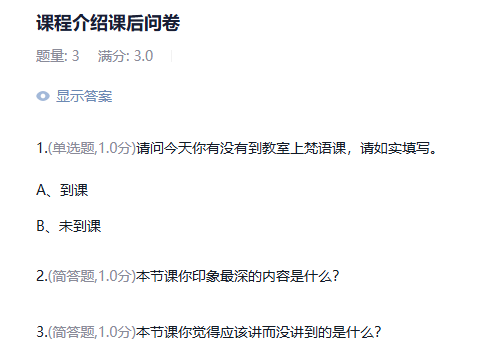
\includegraphics[width=0.9\textwidth]{questionnaire.png}
\end{frame}

\begin{frame}{期末作业样例}
    \centering    
    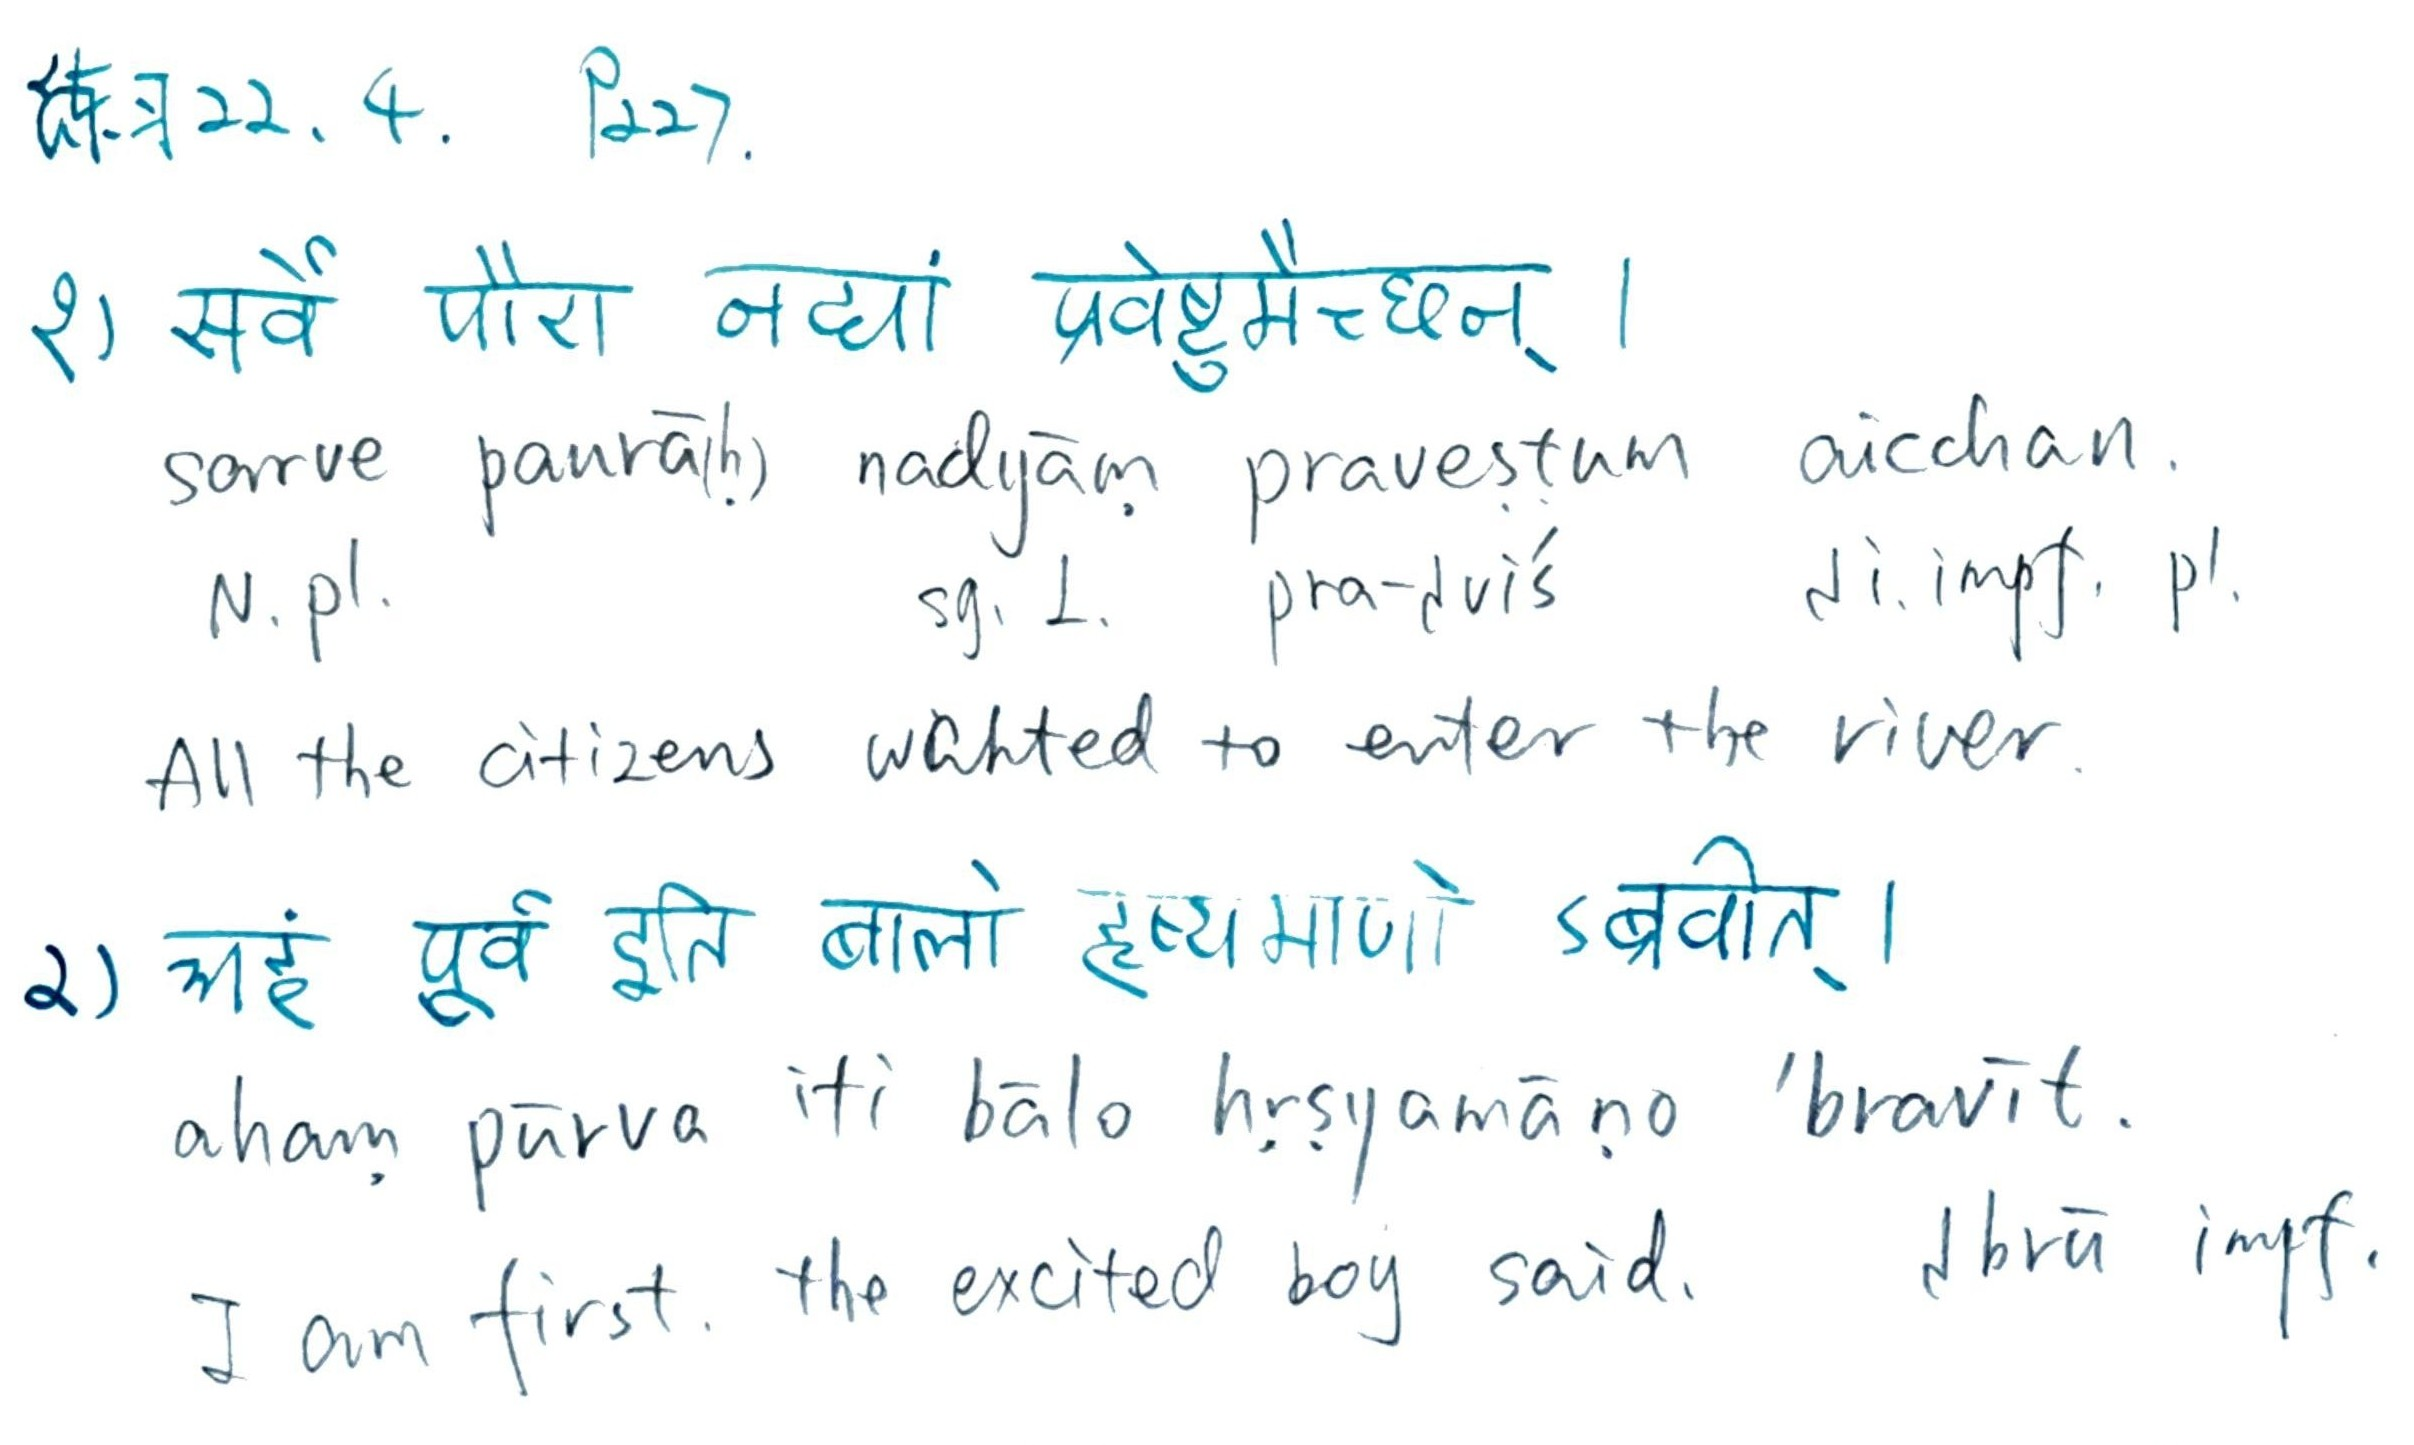
\includegraphics[width=0.9\textwidth]{homework.jpg}
    
    手写拍照、电脑打字,中英文翻译均可 \\
    但最终要求合成一个pdf文档上传
\end{frame}

\section{梵语字母}
\begin{frame}{\insertsection }
    \tableofcontents[currentsection]
\end{frame}

\begin{frame}
  \frametitle{梵语字体}
  \small
  \centering
  \begin{tabular}{@{}lll@{}} % 3 columns    
    天城体(Devanagari)& \skt{saṃskṛta} & 中国 \\
    转写(Transliteration)& Saṃskṛta & \pinyin{Zhong1guo2} \\
    英文(English)& Sanskrit & China \\
  \end{tabular}
\end{frame}

\subsection{元音}

\begin{frame}{\insertsubsection }
  %\small
  \begin{itemize}
    \item
      字母排列总则:发音部位从后往前
    \item
      元音的独立形式:出现在词首
  \end{itemize}
  \bigskip

    \begin{tabular}{@{}llllllll@{}} % 7 columns: type, length/type, and 5 vowels
      简单元音 & \skttrans{a} & \skttrans{ā} & \skttrans{i} & \skttrans{ī} & \skttrans{u} & \skttrans{ū} \\
       & \skttrans{ṛ} & \skttrans{ṝ} & \skttrans{ḷ} & & & \\
    \end{tabular}

    复合元音 ~\skttrans{e} ~\skttrans{ai} ~\skttrans{o} ~\skttrans{au}
\end{frame}

\begin{frame}{发音部位}
    \centering    
    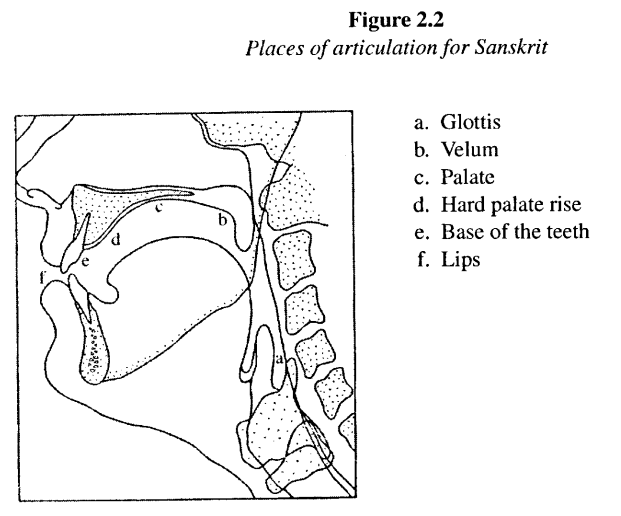
\includegraphics[width=0.9\textwidth]{placeofarticulation.png}
\end{frame}

\subsection{辅音}

\begin{frame}{\insertsubsection }
  \small
  \begin{tabular}{@{}llllll@{}} % 6 columns
     & 不送气  & 送气 & 不送气 & 送气 &   \\
     & 清音  & 清音 & 浊音 & 浊音 & 鼻音  \\
    喉音  & \skttrans{ka}  & \skttrans{kha} & \skttrans{ga} & \skttrans{gha} & \skttrans{ṅa} \\
    腭音  & \skttrans{ca}  & \skttrans{cha} & \skttrans{ja} & \skttrans{jha} & \skttrans{ña} \\
    顶音  & \skttrans{ṭa}  & \skttrans{ṭha} & \skttrans{ḍa} & \skttrans{ḍha} & \skttrans{ṇa} \\
    齿音  & \skttrans{ta}  & \skttrans{tha} & \skttrans{da} & \skttrans{dha} & \skttrans{na} \\
    唇音  & \skttrans{pa}  & \skttrans{pha} & \skttrans{ba} & \skttrans{bha} & \skttrans{ma} \\
      &  & &  & &   \\
    半元音  & \skttrans{ya}  & \skttrans{ra} & \skttrans{la} & \skttrans{va} &  \\
    咝音  & \skttrans{śa}  & \skttrans{ṣa} & \skttrans{sa} &  \skttrans{ha} & \\
  \end{tabular}
\end{frame}

\subsection{学习资料}
\begin{frame}{\insertsubsection }
  \begin{itemize}
    \item
      课本第366-372页附录1
    \item
      \href{https://hindibhasha.com/hindiscripttutor.htm}{课本推荐的练习网站 by SOAS}
    \item
      多邻国软件印地语课程字母部分
  \end{itemize}
\end{frame}  

\section{本节作业}

\begin{frame}{\insertsection }
  \begin{itemize}
    \item
      仔细考虑要不要选课
    \item
      自行练习读写梵语字母
    \item
      \textcolor{gray}{阅读教材第0-2课相关内容}
    \bigskip
    \item
      现在请做学习通\nobreakdash-章节\nobreakdash-课后问卷
  \end{itemize}
\end{frame}  

\end{document}	
